% Slug: four-of-diamonds
% Description: ?
% Author: Cisco
% Story: Cisco
% Test Data: Cisco
% Testers: ?
% Editorial: ?
% TempSlug: four-of-diamonds

% Please don't modify or delete TempSlug

\problem{The Parlor}
Herbert S. Sinclair is developing a suite of puzzles to challenge his grand-nephew Simon Jones, who will be visiting his manor within the coming months.  Each room in his manor has a distinct gimmick, and the style of puzzle to be placed in The Parlor is as follows.

There are three boxes of three different colors: blue, white, and black, laid out in a row in that order.  Each box has a statement written on it.
\begin{center}
    
\includegraphics[width=0.7\linewidth]{img/parlor-boxes.png}

    \textit{Image taken from PC Gamer}
\end{center}

In the room, one would find the following note, explaining the rules of the game:
\begin{center}
    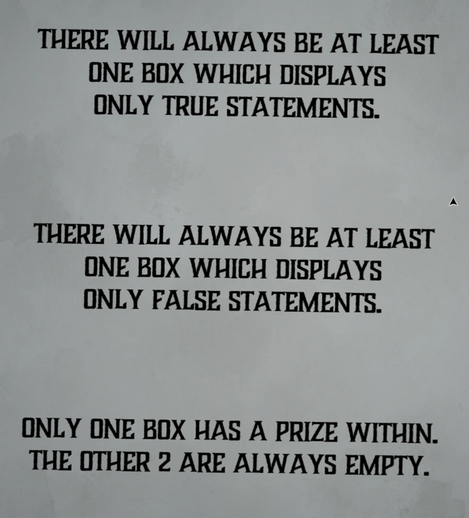
\includegraphics[width=0.3\linewidth]{img/parlor-notes.png}

    \textit{Image taken from the Blue Prince wikia}
\end{center}
Each statement in the room is of one of the following forms:

\begin{itemize}
    \item \texttt{The gems <'are' | 'are not'> in the <'blue' | 'white' | 'black'> box.}
    \item \texttt{The statement on the <'blue' | 'white' | 'black'> box is <'true' | 'false'>.}
    \item \texttt{The statement on the box with the gems is <'true' | 'false'>.}
    \item \texttt{The statements on the empty boxes are both <'true' | 'false'>.}
    \item \texttt{Exactly one box has a statement that is <'true' | 'false'>.}
    \item \texttt{Exactly two boxes have a statement that is <'true' | 'false'>.}
\end{itemize}

The gems, of course, are the prize.  Simon must deduce which box contains the gems.

You have been hired as a playtester for the parlor puzzle.  Given statements that would be placed on these boxes, determine if they have a unique solution, admit multiple solutions, or are paradoxical.  Additionally, if they admit a unique solution, determine which box contains the gems.

\subsection*{Input Format}

The first line of input contains a single integer $T$, the number of test cases.  Then, the descriptions of the $T$ test cases follow.

Each test case is described by four lines: the statement on the blue box, then the statement on the white box, then the statement on the black box, and finally a ``separator'' line consisting of the \texttt{-} character repeated $75$ times.


\subsection*{Output Format}

Output the answer to each test case in its own line.
\begin{itemize}
    \item If---according to the rules of the game---it should have been impossible for the boxes to display these statements, output \texttt{PARADOX}
    \item If the answer can be uniquely deduced from the statements (and the rules of the game), output the color of the box with the gems: one of \texttt{blue} or \texttt{white} or \texttt{black}
    \item If the given statements (and rules of the game) do not determine a unique answer, output \texttt{AMBIGUOUS} instead.
\end{itemize}

\subsection*{Constraints}

\textit{Your program will only be tested on data that satisfies the following constraints.}

% Set to 10^5 in true bounds
\constraints{
    $1 \leq T \leq 400$ \\
    Each statement exactly follows one of the above formats. \\
}

\textit{There is no need to validate in your program that these constraints hold.}

\subsection*{Sample I/O}

\begin{sampleIO}
\begin{verbatim}
TODO
\end{verbatim}
&
\begin{verbatim}
TODO
\end{verbatim}
\end{sampleIO}


\subsection*{Explanation}
Suppose the statement on the white box is false.
\begin{itemize}
\item This directly tells us that the statement on the blue box is false.
\item There must be a true statement, so the statement on the black box must be the true one.
\item Because the statement on the blue box is \textit{false}, we conclude that the gems are in a box with a true statement.
\item So, the gems are in the black box!
\item But... if the black box were true, then the gems \textit{should} be in the blue box.
\item This is a \textbf{contradiction}, so we conclude that the statement on the white box is true.
\end{itemize}

On the other hand, suppose the statement on the white box is true.
\begin{itemize}
\item This directly tells us that the statement on the blue box is true.
\item There must be a false statement, so the statement on the black box must be the false one.
\item Because the statement on the blue box is \textit{true}, we conclude that the gems are in a box with a false statement
\item The statement on the black box (that the gems are in the blue) was indeed false!
\end{itemize}


On the other hand suppose the statement 